\section{Relative Contrast}
The relative contrast (Ctr) values across various dimensions and Lp norms highlight
the significant impact of dimensionality on the behavior of distance measures. As
observed, the contrast starts very high for small dimensions (e.g., $k=2$) and
decreases as dimensionality increases. For example, for $p=0.5$, the contrast begins
at 27.46 for $k=2$ and gradually converges toward a value around 0.435 when $k=300$,
demonstrating that the differences between the farthest and nearest points diminish
as dimensionality increases. This reduction in contrast aligns with the general
understanding of the curse of dimensionality, where the concentration of distances
in high dimensions makes it harder to distinguish between near and far points. The
trend is similarly observed for other $p$ values, such as $p=1$, $p=2$, and $L_{\infty}$,
though the specific rate of decrease varies.

\begin{figure}
    \centering
    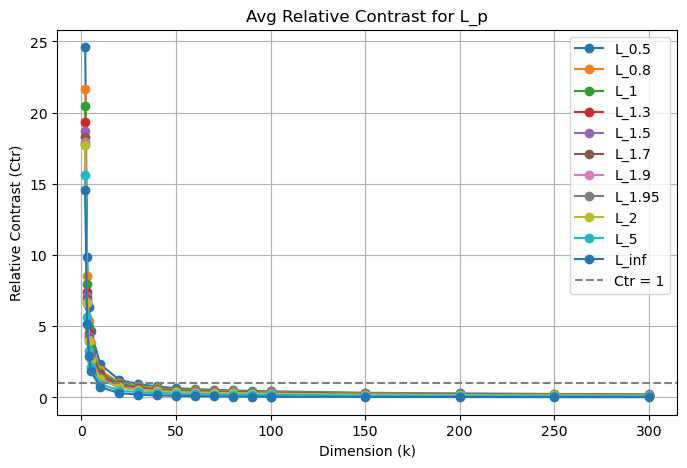
\includegraphics[width=\textwidth, height=\textheight, keepaspectratio]
    {relative-constrast.png}
    \caption{\emph{Avg Relative Contrast} for $L_p$}\label{fig:ctr}
\end{figure}

It can be seen from a closer look of the~\autoref{fig:ctr}, different Lp norms reveals that
larger $p$ values tend to produce lower
Ctr values in high-dimensional spaces, indicating that higher norms concentrate distances
more effectively. For instance, in the case of $L_{\infty}$, the Ctr value decreases from
22.29 at $k=2$ to 0.276 at $k=300$, showing a clear convergence trend. Specifically, for
higher $p$ values like $p=2$, the contrast appears to converge around a value of 0.31 as
$k$ approaches 300. Lower $p$ norms, such as $p=0.5$, approach a final contrast value of
approximately 0.435. These values reflect the final state as distances become nearly uniform
at high dimensions. The decrease in contrast across all norms points toward the saturation of
distance values in higher dimensions, where distances become relatively similar. In particular,
the lower $p$ norms like $p=0.5$ show higher initial contrast, reflecting their sensitivity to
small variations, while the convergence rate tends to stabilize more gradually compared to higher
$p$ values. These findings highlight how Lp norms influence the spread of distances in
high-dimensional spaces, with larger $p$ values converging more quickly to a $0$ contrast which makes
it more difficult to discern the distances between the data points.

